% Created 2022-07-09 Sat 18:37
% Intended LaTeX compiler: pdflatex
\documentclass[titlepage,a4paper]{article}
\usepackage[utf8]{inputenc}
\usepackage[T1]{fontenc}
\usepackage{graphicx}
\usepackage{longtable}
\usepackage{wrapfig}
\usepackage{rotating}
\usepackage[normalem]{ulem}
\usepackage{amsmath}
\usepackage{amssymb}
\usepackage{capt-of}
\usepackage{hyperref}
\usepackage{minted}
\hypersetup{colorlinks=true,linkcolor=black,urlcolor=blue,bookmarksopen=true}
\usepackage{a4wide}
\usepackage{bookmark}
\usepackage{fancyhdr}
\usepackage[spanish]{babel}
\usepackage[utf8]{inputenc}
\usepackage[T1]{fontenc}
\usepackage{graphicx}
\usepackage{float}
\usepackage{minted}
\usepackage{svg}
\pagestyle{fancy}
\fancyhf{}
\fancyhead[L]{TP2 - Grupo 22}
\fancyhead[R]{Algoritmos y Programacion III - FIUBA}
\renewcommand{\headrulewidth}{0.4pt}
\fancyfoot[C]{\thepage}
\renewcommand{\footrulewidth}{0.4pt}
\usemintedstyle{stata-light}
\newminted{c}{bgcolor={rgb}{0.95,0.95,0.95}}
\usepackage{color}
\usepackage[utf8]{inputenc}
\usepackage{fancyvrb}
\fvset{framesep=1mm,fontfamily=courier,fontsize=\scriptsize,numbers=left,framerule=.3mm,numbersep=1mm}
\usepackage[nottoc]{tocbibind}
\date{\today}
\title{}
\hypersetup{
 pdfauthor={},
 pdftitle={},
 pdfkeywords={},
 pdfsubject={},
 pdfcreator={Emacs 29.0.50 (Org mode 9.5.4)}, 
 pdflang={Spanish}}
\begin{document}

\begin{titlepage}
    \hfill
\includegraphics[width=6cm]{logofiuba.jpg}
    \centering
    \vfill
    \Huge \textbf{Trabajo Práctico 2 — GPS Challenge}
    \vskip2cm
    \Large [75.07/95.02] Algoritmos y Programación III \\
    Primer cuatrimestre de 2022\\
    \vfill
    \begin{tabular}{ | l | l | l | }
      \hline
      Alumno & Padron & Email \\ \hline
      CASTILLO, Carlos & 108535 & ccastillo@fi.uba.ar \\ \hline
      DEALBERA, Pablo Andres & 106585 & pdealbera@fi.uba.ar \\ \hline
      RECCHIA, Ramiro & 102614 & rrecchia@fi.uba.ar \\ \hline
    \end{tabular}
    \vfill
    \begin{tabular}{ | l | l | }
      \hline
      Corrector & Email \\ \hline
      GOMEZ, Joaquin & gjoaquin@fi.uba.ar \\ \hline
      VALDEZ, Santiago & vsantiago@fi.uba.ar \\ \hline
    \end{tabular}
    \vfill
\end{titlepage}
\tableofcontents
\newpage
\definecolor{bg}{rgb}{0.95,0.95,0.95}

\section{Supuestos}
\label{sec:orgc3132fc}

\section{Diagramas de clases}
\label{sec:orga1c5731}
\subsection{Vehiculo}
\label{sec:org70eef3c}

\begin{center}
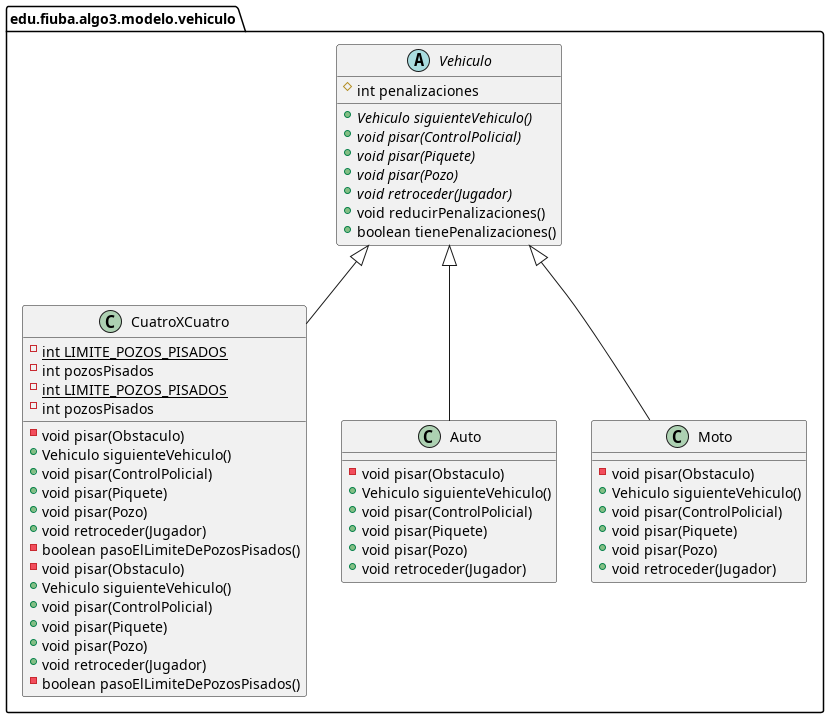
\includegraphics[width=.9\linewidth]{./diagramas/clases-vehiculo.png}
\end{center}

\subsection{Sorpresas}
\label{sec:orgf88f136}

\begin{center}
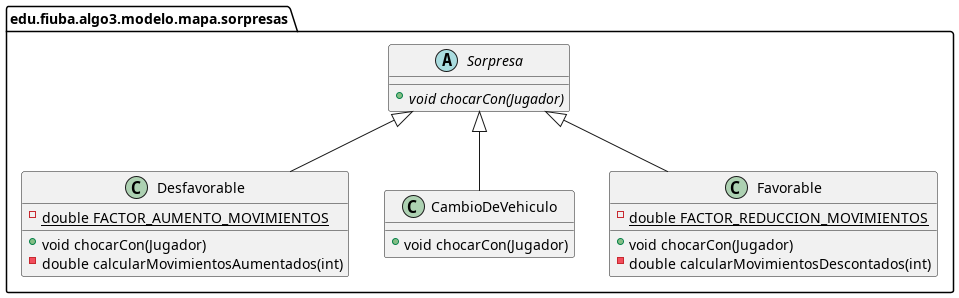
\includegraphics[width=.9\linewidth]{./diagramas/clases-sorpresas.png}
\end{center}

\subsection{Obstaculos}
\label{sec:org72cb2eb}

\begin{center}
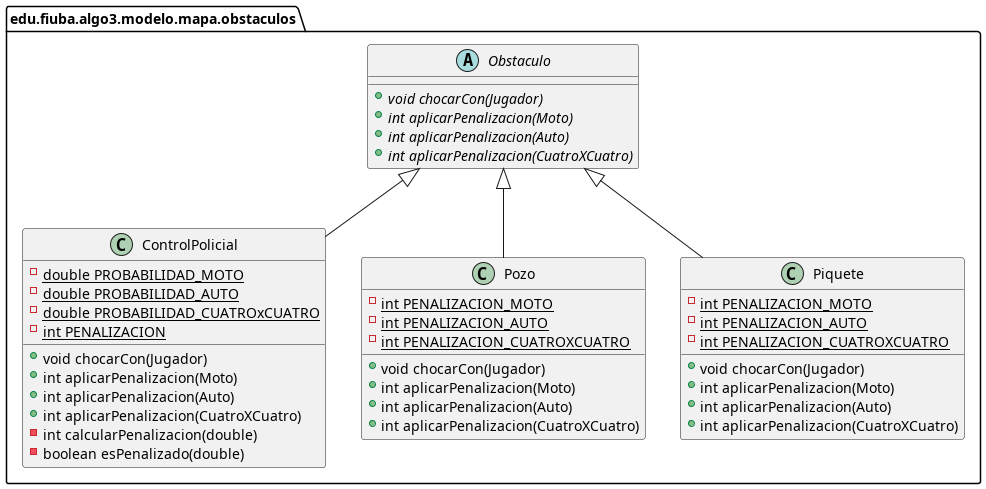
\includegraphics[width=.9\linewidth]{./diagramas/clases-obstaculos.png}
\end{center}

\subsection{Mapa}
\label{sec:org2ec8249}

\begin{center}
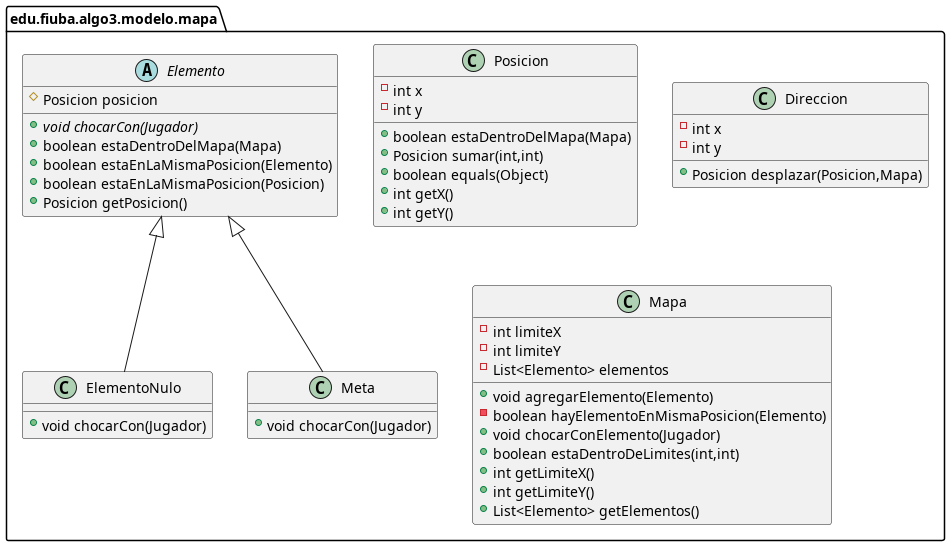
\includegraphics[width=.9\linewidth]{./diagramas/clases-mapa.png}
\end{center}

\subsection{Juego}
\label{sec:org5ee8a3a}

\begin{center}
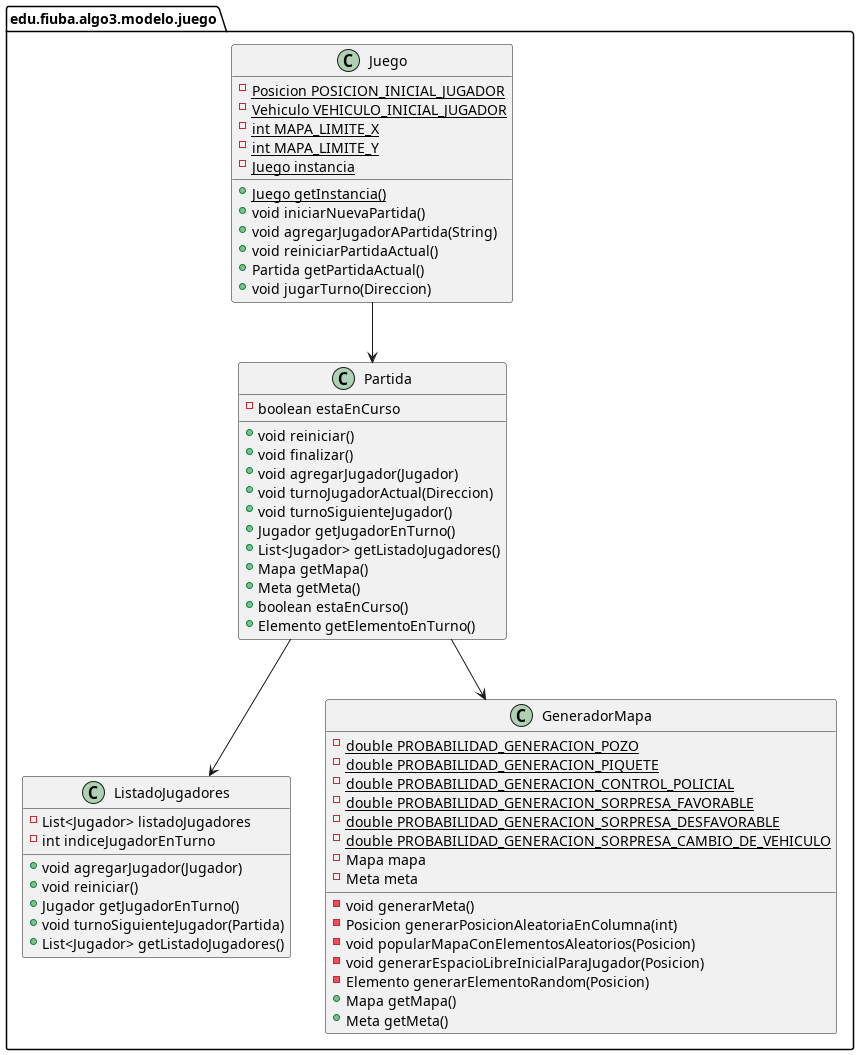
\includegraphics[width=.9\linewidth]{./diagramas/clases-juego.png}
\end{center}

\section{Diagrama de paquetes}
\label{sec:org9a5bad0}
\begin{center}
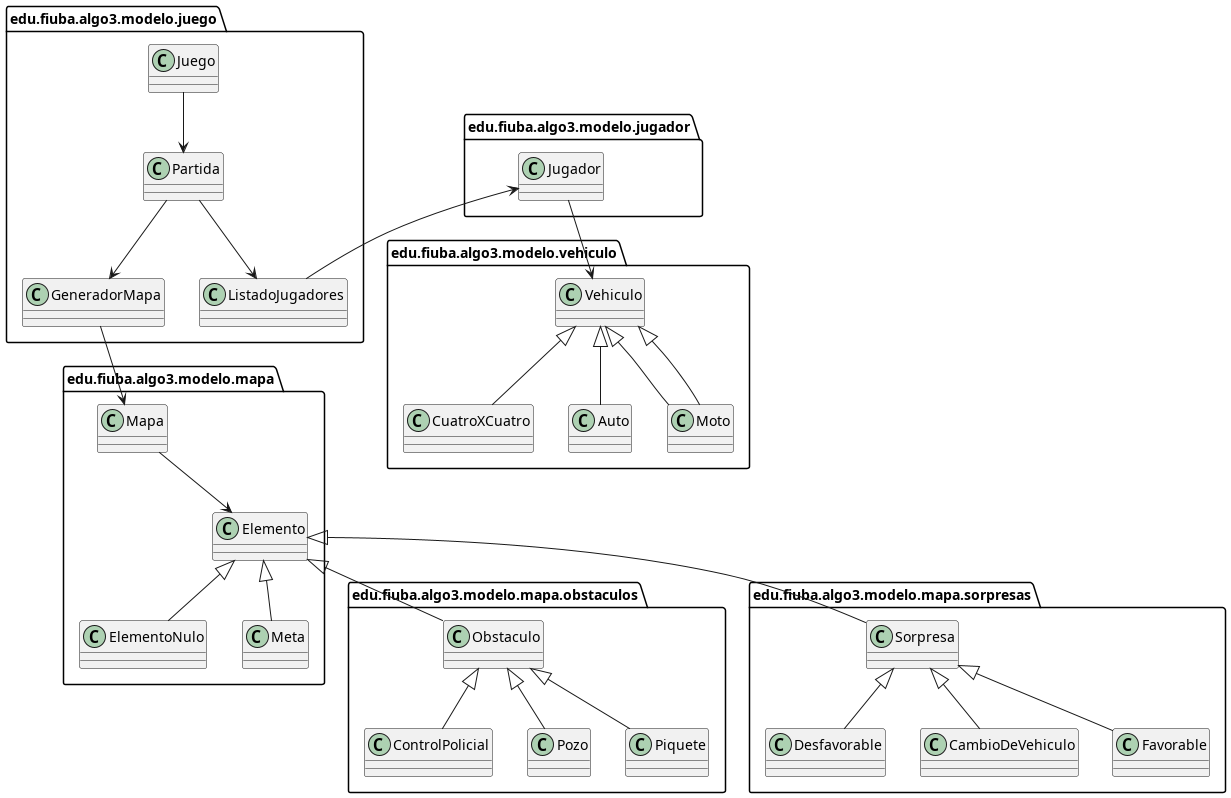
\includegraphics[width=.9\linewidth]{./diagramas/paquetes.png}
\end{center}

\section{Diagramas de secuencia}
\label{sec:org791f04e}
\subsection{Interaccion Jugador - Sorpresa Cambio de Vehiculo}
\label{sec:org2833f76}

\begin{center}
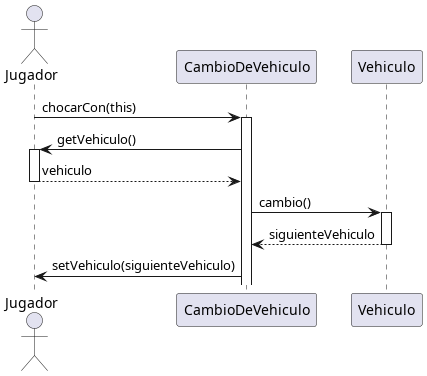
\includegraphics[width=.9\linewidth]{./diagramas/jugadorAvanzaYSeEncuentraConUnaSorpresaCambioDeVehiculo.png}
\end{center}

\subsection{Interaccion Jugador - Sorpresa Favorable}
\label{sec:org6382d36}

\begin{center}
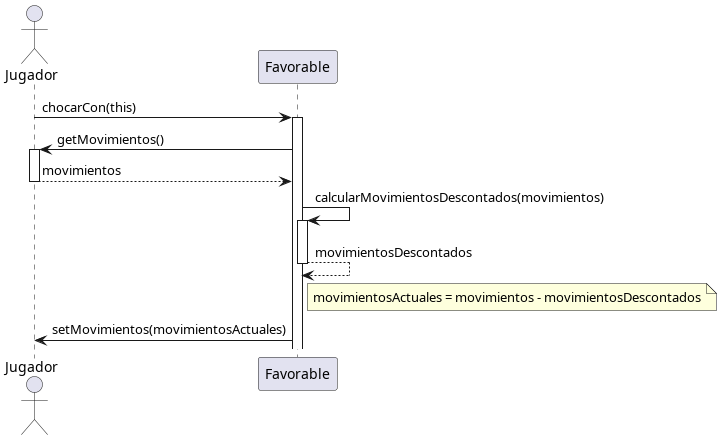
\includegraphics[width=.9\linewidth]{./diagramas/jugadorAvanzaYSeEncuentraConUnaSorpresaFavorable.png}
\end{center}

\subsection{Interaccion Jugador - Elemento}
\label{sec:orgd6b8e9b}

\begin{center}
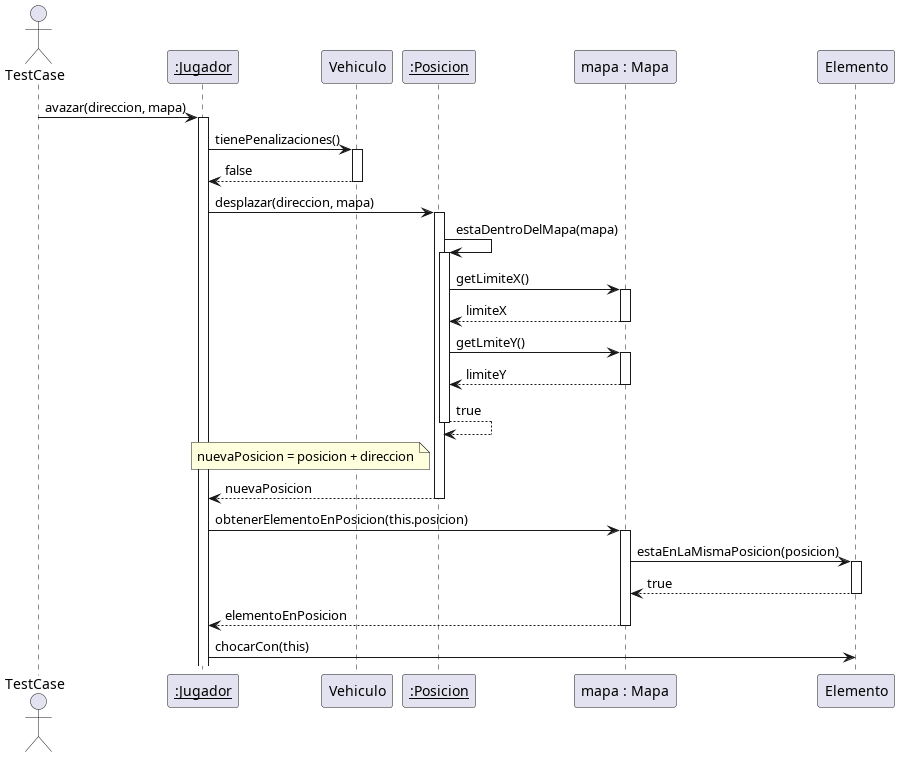
\includegraphics[width=.9\linewidth]{./diagramas/jugadorAvanzaYSeEncuentraConUnElemento.png}
\end{center}

\subsection{Jugador avanza y se encuentra con un Elemento}
\label{sec:orgd8a100d}

\begin{center}
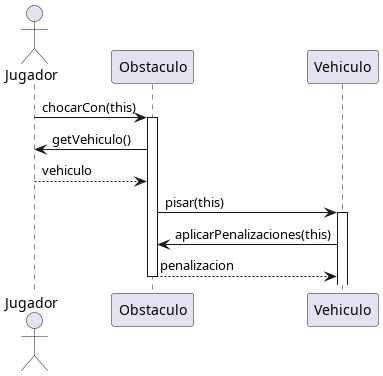
\includegraphics[width=.9\linewidth]{./diagramas/jugadorAvanzaYSeEncuentraConUnObstaculo.png}
\end{center}

\section{Diagramas de estado}
\label{sec:org80f2570}

\section{Detalles de implementación}
\label{sec:org0fa7554}
\subsection{Vehiculo}
\label{sec:orgede4f85}

En principio tenes una clase abstracta llamada \emph{Vehiculo} y usamos herencia para
abstraer comportamiento comun entre su tres clases hijas: Moto, Auto y CuatroXCuatro.

\subsection{Elemento}
\label{sec:orgccc91a2}

Es una clase abstracta de la cual heredan dos clases:

\begin{itemize}
\item Obstaculo
\begin{itemize}
\item Pozo, Piquete y Control Policial.
\end{itemize}
\item Sorpresa
\begin{itemize}
\item Favorable y Cambio de Vehiculo
\end{itemize}
\item Meta
\end{itemize}

Utilizamos esta clase para definir compotamientos que los distintos
Elementos tienen en comun, como por ejemplo que pueden \texttt{chocaCon} un
jugador, y algunas funciones de ayuda para saber si el elemento esta
adentro del mapa, si esta en la misma posicion que otro elemento o una
posicion arbitraria, etc.

\subsection{Interaccion Vehiculo-Obstaculo}
\label{sec:org458b237}

Para la interaccion Vehiculo-Obstaculo decidimos usar el patron \emph{Double
Dispatch} de forma ya que tenemos una interaccion de muchos a muchos entre los
hijos de ambas clases abstractas:

\begin{center}
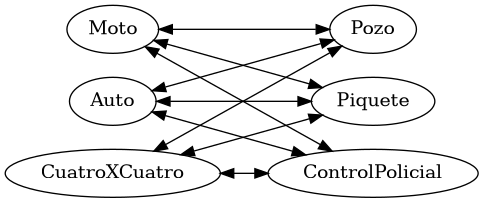
\includegraphics[width=.9\linewidth]{diagramas/interaccionVehiculoObstaculo.png}
\end{center}

Ademas de esto teniamos la necesidad de modelar implementaciones especificas
como el caso de CuatroXCuatro-Pozo donde la CuatroXCuatro debe pisar tres pozos
para recibir una penalizacion, cosa que no sucede en ninguna de las otras interacciones.

Para esto los Vehiculos tienen firmas segun cada implementacion de Obstaculo.
Y cada implementacion de Obstaculo tiene firmas para cada Vehiculo.

\subsection{Ranking y Persistencia}
\label{sec:org3d8da03}

Para el ranking usamos un \texttt{HashMap<String, Long>} con el que
almacenamos como clave el nombre del jugador y como valor la cantidad
de movimientos minimo que hizo.

Esto se maneja en el \texttt{ControladorHistorialPartidas} que tiene dos
metodos que hacen uso de la libreria Gson para crear un JSON del
\texttt{HashMap}, escribirlo en un archivo \texttt{ranking.json} y otro metodo para
obtener el historial en siguientes ejecuciones del programa
\emph{deserializando} el JSON parseado como un \texttt{HashMap} de nuevo.

\begin{minted}[breaklines=true,breakanywhere=true,bgcolor=bg]{json}
{
  "Pablo": 24,
  "Ramiro": 20,
  "Carlos": 30
}
\end{minted}

\section{Excepciones}
\label{sec:orgc5c5dd2}
\subsection{(No) Excepcion cuando el usuario intentar ir fuera del Mapa}
\label{sec:orgc646474}

Una observacion que tuvimos durante el desarrollo fue la posibilidad
de agregar una excepcion cuando el usuario intenta ir fuera de los
bordes del mapa. Nosotros como supuesto elegimos no tratar esto como
un error y directamente el modelo maneja esta posibilidad y no permite
al usuario avanzar por fuera de los limites del mapa.
\end{document}